%%
%% Copyright 2025 Oxford University Press
%%
%% This file is part of the 'oup-authoring-template Bundle'.
%% ---------------------------------------------
%%
%% It may be distributed under the conditions of the LaTeX Project Public
%% License, either version 1.3 of this license or (at your option) any
%% later version.  The latest version of this license is in
%%    https://www.latex-project.org/lppl.txt
%% and version 1.2 or later is part of all distributions of LaTeX
%% version 1999/12/01 or later.
%%
%% The list of all files belonging to the 'oup-authoring-template Bundle' is
%% given in the file `manifest.txt'.
%%
%% Template article for Oxford University Press's document class `oup-authoring-template'
%% with bibliographic references
%%

%%%CONTEMPORARY%%%
\documentclass[unnumsec,webpdf,contemporary,large]{oup-authoring-template}

\graphicspath{{Fig/}}

% line numbers
%\usepackage[mathlines, switch]{lineno}
%\usepackage[right]{lineno}

% --- Tables & figures helpers ---
\usepackage{graphicx}
\usepackage{booktabs}
\usepackage{tabularx}
\usepackage{array}
\usepackage{siunitx}
\usepackage[section]{placeins}
\sisetup{
  detect-all,
  group-separator = {,},
  group-minimum-digits = 4
}
 \sisetup{detect-weight=true, detect-family=true}

\begin{document}

\journaltitle{European Conference on Computational Biology}
\DOI{DOI added during production}
\copyrightyear{2026}
\pubyear{YEAR}
\vol{XX}
\issue{x}
\access{Published: Date added during production}
\appnotes{Paper}

\firstpage{1}

%\subtitle{Subject Section}

\title[VCF-RDFizer]{VCF-RDFizer: A Conversion Tool to Represent Variant Data as a Knowledge Graph}

\author[1,2,$\ast$]{Elias Crum\ORCID{0009-0005-3991-754X}}
\author[1]{Bart Buelens\ORCID{0000-0001-7734-3747}}
\author[2]{Ruben Taelman\ORCID{0000-0001-5118-256X}}
\author[1]{Gökhan Ertaylan\ORCID{0000-0001-5602-6435}}

\address[2]{\orgdiv{IDLab, Department of Electronics and Information Systems}, \orgname{Ghent University -- imec}, \orgaddress{\street{Technologiepark-Zwijnaarde 116}, \postcode{9052}, \country{Belgium}}}
\address[1]{\orgdiv{Digital Biological Systems}, \orgname{Flemish institute for Technological Research (VITO)}, \orgaddress{\street{Boeretang 200}, \postcode{2400}, \country{Belgium}}}

\corresp[$\ast$]{Corresponding author. \href{email:ecrum@ugent.be}{E-mail: ecrum@ugent.be}}

\received{Date}{0}{Year}
\revised{Date}{0}{Year}
\accepted{Date}{0}{Year}

%\editor{Associate Editor: Name}

%\abstract{
%\textbf{Motivation:} .\\
%\textbf{Results:} .\\
%\textbf{Availability:} .\\
%\textbf{Contact:} \href{name@email.com}{name@email.com}\\
%\textbf{Supplementary information:} Supplementary data are available at \textit{Journal Name}
%online.}

\abstract{%
The Variant Call Format (VCF) is the de facto standard for representing human genomic variation and underpins large-scale population genomics, clinical sequencing, and precision medicine initiatives. As uses for VCF data expand, so do opportunities to enrich variant data through integration with complementary resources without modifying the VCF specification itself. Such enrichment may include additional metadata, sample- or patient-level information, test results, links to public databases, or privacy-related annotations. To accommodate the structured and scalable linkage of these heterogeneous data, we see promise in the use of a knowledge graph representation via the Resource Description Framework (RDF). To benefit from the potential of RDF, the initial challenge is translating VCF file data into RDF. Here, we present VCF-RDFizer, a command-line tool available on PyPI and Conda-Forge that provides an end-to-end pipeline for converting VCF into RDF. VCF-RDFizer introduces a publicly available vocabulary that models VCF constructs while integrating established ontologies from biomedical knowlge graphs. The tool preserves variant-level detail, genotype information, and metadata, enabling semantically an enriched and standards-aware representation of genomic variation. Unlike ad hoc or partial transformations, VCF-RDFizer offers a systematic and reproducible workflow from raw VCF to structured RDF and full coverage of all data represented in VCF files. To assess the feasibility of our tool, we tested VCF-RDFizer on six publicly available VCF files of varying sizes and complexities. Our evaluation demonstrates that conversion is tractable across realistic dataset scales and can be performed successfully on standard hardware. By transforming VCF into an interoperable knowledge graph format, VCF-RDFizer lays the foundation for the exciting possibilities of heterogeneous data enrichment of VCF.%
}

\keywords{Knowledge Representation, Genomic Mutation Data, Semantics}

\maketitle

\section{Introduction}

%% VCF Intro - what is it? how can we improve its usage?
The Variant Call Format (VCF) is the dominant standard for genomic variant exchange across research and clinical pipelines, including pharmacogenomics and precision medicine applications \cite{vcf_spec_2024,mcleod_cancer_2013,souche_recommendations_2022}. 
As its adoption has expanded, downstream applications increasingly require integration of variant calls with additional contextual information, including sample- and patient-level descriptors, phenotype associations, external database references, and policy annotations governing data access. 
This requirement is already visible in operational semantic-genomics efforts that connect variant data to external knowledge resources and structured governance layers for controlled access \cite{togovar_2022,sphn_semantic_2023,acl_2021}.
Consequently, practical analysis workflows would increasingly benefit from query models that can combine variant facts, linked biomedical context, and access constraints.

While VCF provides a compact and expressive encoding of genomic variation, it was not designed as a general-purpose semantic integration framework for linking heterogeneous data sources.
These limitations become particularly apparent in domains such as privacy protection, where fine-grained and machine-interpretable access control mechanisms are desirable. 
In other domains, frameworks such as the Open Digital Rights Language (ODRL) \cite{odrl_2018} enable granular policy expression directly linked to data resources. 
Representing variant data in a form that can accommodate similar policy annotations would support controlled access and governance use cases; however, the VCF syntax offers no natural mechanism for expressing such structured constraints. 
More broadly, querying VCF data at scale, such as retrieving subsets of variants by genomic region or annotation criteria, typically relies on specialized command-line utilities (e.g., bcftools, htslib) or custom processing pipelines rather than declarative, interoperable query mechanisms.

%% RDF Intro - What is it? How can it help enrich VCF data?
Representing VCF data using the Resource Description Framework (RDF) \cite{rdf} provides a principled solution to enriching VCF data and expanding its usage. 
RDF models data as a graph of explicitly defined entities and relationships identified by machine-readable globally unique identifiers (IRIs) \cite{rdf}.
This representation strategy enables (i) structured linkage between variant data and external biomedical resources \cite{bio2rdf_2008,sib_swiss_institute_of_bioinformatics_rdf_group_members_sib_2024}, (ii) native declarative and expressive querying over graph-structured data via the SPARQL query language \cite{sparqllang}, and (iii) unique methods of fine-grained privacy policy enforcement over VCF data and linkages \cite{odrl_2018,acl_2021}.
Practically, when combined, RDF representations of VCF files could enable complex, expressive queries that span variant data and linked resources, such as "find all VCF records (in a given database) whose "ALT" alleles in gene X that are annotated with phenotype Y and have access restrictions Z".

%% How do we turn VCF into RDF? Why is it hard?
Converting VCF into RDF requires \textit{semantic lifting}, which means transforming row-based file content into machine-interpretable graph statements.
In practical terms, each relevant VCF element (e.g., variant, allele, genotype, sample) is given a stable global identifier (an IRI), and each data field is converted into RDF facts of the form subject--predicate--object (triples), where the predicate defines the relationship type.
Using ontology-aligned predicates ensures that these relationships have consistent meaning across datasets, so the final RDF graph can be queried and linked reliably.
This conversion process contains two important components: 1) the vocabulary and semantic schema for defining IRIs that represent particular VCF file data entries, and 2) a computational process that maps the vocabulary terms to the recorded data within a VCF file.
Crucially, this conversion process must be systematic and reproducible rather than file-specific or hard-coded, particularly given the variability in VCF header declarations and field definitions.

Although VCF adheres to a formal specification \cite{vcf_spec_2024}, its structure permits substantial heterogeneity across datasets. 
INFO fields often contain semi-structured or multi-valued annotations; FORMAT and genotype columns may differ in composition and semantics between files; alternate allele representations extend beyond simple SNPs to complex structural variants; and metadata header lines introduce dataset-specific definitions. 
Multi-sample VCF files further increase structural complexity by aggregating per-sample genotype information within a shared variant record.
This combination of flexibility and heterogeneity complicates the construction of a uniform semantic representation and necessitates carefully designed, ontology-aware transformation logic to ensure consistency, scalability, and reproducibility.
Thus, both defining a semantic vocabulary to describe VCF file contents and designing a computational conversion process that accurately assigns semantic IRIs to VCF file data fields are non-trivial challenges.

%% What VCF as RDF work has been done before? (Related Work)
Prior semantic genomics efforts provide important foundations but do not yet offer a general, reproducible VCF-to-RDF tooling that comprehensively converts all fields represented in VCF files into an RDF representation.

Existing conversion tools that offer solutions for the VCF-to-RDF conversion process include VCF2RDF within TOGOvar \cite{togovar_2022}, JVarKit VcfToRdf, the ruby-rdf/rdf-vcf library, and the semantic beacons implementation \cite{semantic_beac_2025}. 
While these efforts demonstrate the feasibility of representing genomic variants in RDF, they typically model only subsets of VCF semantics, provide limited support for genotype and metadata fields, rely on custom parsing logic, or are embedded within specialized infrastructures rather than offering a standalone, reproducible transformation pipeline.
Another notable but limited strategy for VCF-to-RDF translation involves manually combining existing ontologies with YAML-based transformation rules \cite{yaml-spec_2025}, as demonstrated in semantic beacon workflows \cite{semantic_beac_2025}. 
While effective for simple elements, such rule-based approaches struggle to model deeply nested, dataset-specific structures and therefore lack generalizability across diverse VCF datasets.

Along with tools for RDF conversion, a substantial body of ontological work supports semantic modeling of genomic data. 
The GA4GH variant schema \cite{ga4gh_varschema_2021} provides a structured representation of human genomic variants, while FALDO \cite{faldo_2016} standardizes genomic coordinate modeling and the Sequence Ontology (SO) \cite{seq_ont_2005} defines controlled vocabularies for sequence features and variant types. 
Extensions such as GENO and SNPO \cite{seq_ont_2005} address genotype and sample-level semantics. 
Domain-specific resources including TOGOvar \cite{togovar_2022}, HERO \cite{hero-genomics_2025}, and the SPHN multi-omics schema \cite{sphn_semantic_2023} further enrich variant representation, particularly for clinically oriented applications. 
Collectively, these vocabularies model important facets of VCF data but do not themselves provide a comprehensive and reproducible transformation mechanism from arbitrary VCF files.

Other large-scale RDF integration initiatives, including Bio2RDF \cite{bio2rdf_2008} and OpenBioLink \cite{openbiolink_2019}, demonstrate the potential of knowledge graph approaches for biomedical data integration, including variant-related information. 
However, their focus lies in curated database integration or downstream learning tasks rather than full semantic coverage of heterogeneous VCF constructs. 
Across prior efforts, challenges remain regarding completeness, extensibility, tooling robustness, and support for the flexible structures found in INFO, FORMAT, GENOTYPE, and HEADER fields.

%% Why not use mapping language to mediate conversion (also makes things easily customizable + reproducible)
Given the heterogeneity of VCF file structure and the need for reproducible, extensible transformation logic, declarative mapping languages provide a principled strategy for VCF-to-RDF conversion. 
Rather than embedding dataset-specific parsing rules in custom code, mapping languages allow conversion logic to be expressed as reusable, transparent rules that can be shared and adapted across workflows.

In the larger semantic web technology space, several declarative frameworks have been developed for mapping heterogeneous or semi-structured data to RDF. 
Early approaches include TARQL \cite{tarql}, which supports SPARQL-based transformations of tabular data, and tools such as SDM-RDFizer \cite{sdm-rdfizer_2020}, which prioritize high-performance ingestion of large datasets. 
For semi-structured data RML (RDF Mapping Language) \cite{rml_2024}, an extension of R2RML \cite{r2rml_2012}, supports non-relational and semi-structured data source conversion, making it well suited to the irregular and nested structure of VCF files. 
Its ecosystem includes execution engines such as rmlmapper \cite{rmlmapper-java_2025} and RMLStreamer \cite{rmlstreamer_2022}, supporting both local and scalable processing environments.

RML's design makes it particularly suitable for the VCF format, whose INFO, FORMAT, GENOTYPE and HEADER fields vary in structure and cardinality across files and datasets. 
Its rule-based, declarative mapping model allows users to encode domain semantics explicitly while adapting to the heterogeneous structure of genomic data, and its ecosystem—including rmlmapper and the distributed engine RMLStreamer—aligns well with FAIR data workflows and scalable transformation pipelines. 
Among existing tools, RML provides a uniquely extensible approach for modeling the semi-structured and complex fields present in VCF, offering a natural path toward generating reusable semantic representations.

%% Acknowledgment of RDF Inflation and the strategies to address it
A well-recognized trade-off of RDF representation is semantic inflation: the increase in storage size that results when compact, semi-structured formats such as VCF are expanded into explicit subject–predicate–object triples. 
In our benchmark, this expansion was substantial: raw RDF outputs were approximately 30.8--80.4$\times$ larger than the corresponding input \texttt{.vcf.gz} files (Table~\ref{tab:conversion-stats}).
This expansion is amplified by the use of fully qualified IRIs and the materialization of implicit relationships as explicit graph edges \cite{rdf}.

RDF can be serialized in formats such as N-Triples or N-Quads \cite{nquads_2014}, which are simple, line-oriented representations well suited for streaming and large-scale processing. 
However, their verbosity makes compression essential for practical storage. 
General-purpose compressors, more useful for long-term storage, such as gzip routinely reduce RDF file sizes by more than 90\%, while Brotli \cite{brotli_2019} often achieves higher compression ratios with modest additional computational overhead.
Beyond byte-level compression, HDT (Header–Dictionary–Triples) \cite{hdt_2013} provides a domain-specific binary representation of RDF that incorporates dictionary encoding and indexing structures. 
HDT not only substantially reduces storage requirements but also enables query execution directly over the compressed representation, avoiding full decompression. 
For archival scenarios, HDT files may be further compressed using gzip or Brotli to maximize storage efficiency.
Together, these complementary strategies can reduce the storage overhead introduced by semantic inflation while preserving the interoperability and query capabilities that motivate RDF-based genomic data representation.

%% So what + Aims of study
In this study, we aim to provide an end-to-end, reproducible command-line pathway from VCF to serialized, compressed RDF through the python-based tool VCF-RDFizer: \url{https://github.com/ecrum19/VCF-RDFizer}. 
Specifically, we (i) define a public VCF-RDFizer vocabulary to sematically define VCF file entry data that is aligned with established ontologies: \url{https://w3id.org/vcf-rdfizer/vocab\#}, (ii) implement customizable RML conversion mappings that preserve variant-, genotype-, and metadata-level information, and (iii) evaluate conversion performance of nine public VCF files using VCF-RDFizer, including runtime, memory, output scale, and compression behavior: \url{https://github.com/ecrum19/vcf-rdfizer-testing}.


\section{VCF-RDFizer CLI Tool}\label{sec2}
VCF-RDFizer is a command-line workflow that converts input VCF files into semantically enriched RDF using a reproducible mapping pipeline. 
The workflow integrates parsing, mapping, validation, and optional compression in one execution path. 
An overview is shown in Figure~\ref{fig1}.

\begin{figure*}
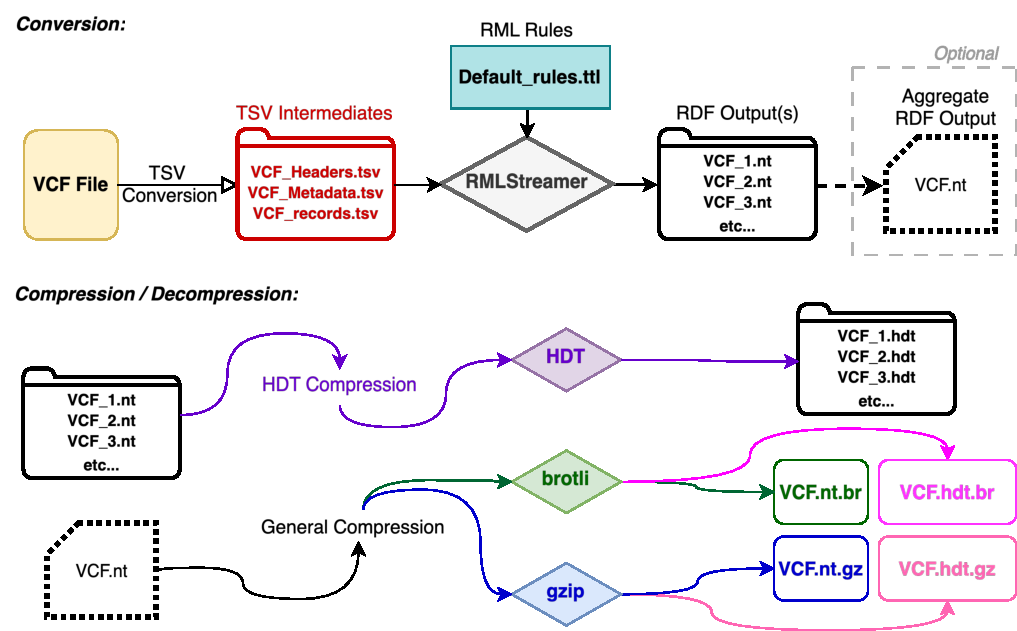
\includegraphics[width=0.9\textwidth]{vcf2rdf.pdf}
\caption{\textbf{VCF-RDFizer Pipeline Workflow}
The flowchart depicts end-to-end conversion from VCF input to semantically enriched, compressed RDF outputs.
\textbf{Conversion}: VCF-RDFizer parses converts VCF file into CSV intermediates, uses RML mappings and RMLStreamer to generate N-Triples, optionally aggregates VCF RDF outputs to a single .nt file. 
\textbf{Compression}: VCF-RDFizer compresses RDF output(s) via HDT and/or General Compression (gzip, Brotli) for downstream storage and querying.
HDT compressed RDF files can also be further compressed via general compression (either gzip or Brotli).
\textbf{Decompression}: All steps in the compression workflow are reversible.
} \label{fig1}
\end{figure*}

\subsection{Semantic Model}\label{subsec2.1}
The semantic model combines a dedicated VCF-RDFizer vocabulary (\url{https://w3id.org/vcf-rdfizer/vocab#}) with established ontologies to maximize interoperability and reuse.
Genomic coordinates are represented with FALDO \cite{faldo_2016}, variant typing aligns with the Sequence Ontology \cite{seq_ont_2005}, and genotype/sample constructs are aligned with existing genomics vocabularies (including HERO where applicable) \cite{hero-genomics_2025}.
This hybrid strategy retains VCF-specific semantics while avoiding duplication of mature ontology terms.

The model preserves three information layers: variant-level assertions, genotype/sample assertions, and metadata/header assertions.
Core entities are minted using deterministic IRI templates derived from stable VCF attributes (e.g., chromosome, position, reference allele, alternate allele), which keeps identifiers reproducible across runs.
When provenance or context separation is required, statements can be organized into named graphs while maintaining a unified SPARQL query surface.

\begin{figure*}
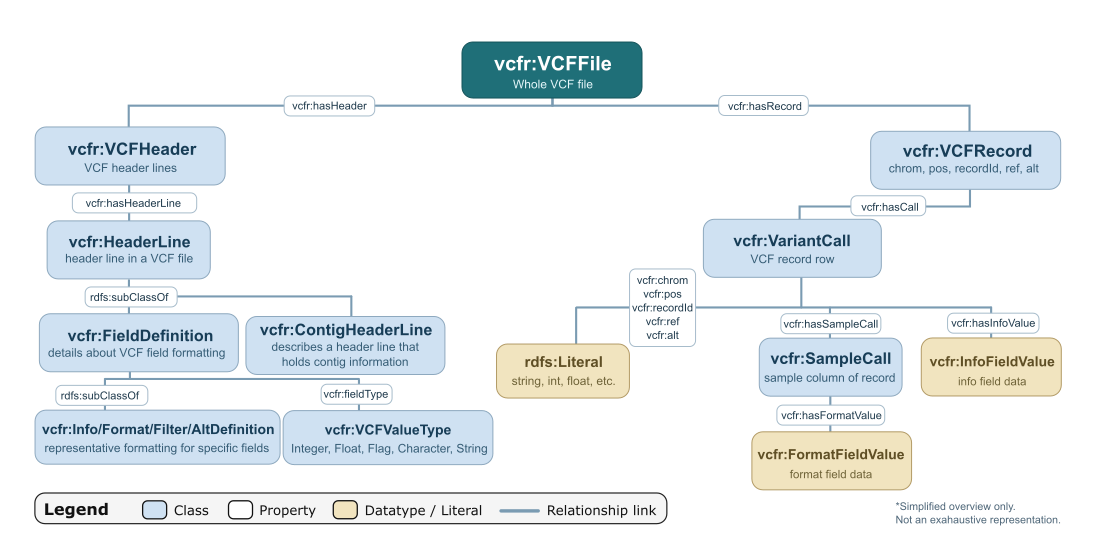
\includegraphics[width=0.9\textwidth]{class-hierarchy-paper.png}
\caption{\textbf{Semantic VCF Vocabulary (sample)}
The figure depicts a simplified representation of the semantic heirarchy for representation of the data within a VCF file.
All prefixes \textit{vcfr:} are an abbreviation for \url{https://w3id.org/vcf-rdfizer/vocab\#} .
A companion website was created for a more complete, detailed, and interactive representation of this vocabulary.
Website available at: \url{https://ecrum19.github.io/VCF-RDFizer-vocabulary/}.
} \label{fig2}
\end{figure*}


\subsection{Tool Workflow}\label{subsec2.2}
VCF-RDFizer is implemented as a CLI pipeline with four stages: 
(1) VCF conversion to TSV, 
(2) TSV conversion to RDF via RML mappings and RMLStreamer, 
(3) RDF validation and optional output aggregation, 
and (4) optional compression and run statistics outputs. 
The pipeline preserves metadata and genotype content rather than discarding it during preprocessing. 
Outputs are emitted as N-Triples by default, with various optional arguments to mediate formatting and/or compression.

Mappings are authored in Turtle as modular RML rule sets that cover fixed VCF columns, variable INFO attributes, FORMAT/genotype structures, and metadata declarations. 
This modularity allows rules to be extended per annotation family without rewriting the full pipeline. 
Subject generation, predicate-object assertions, datatypes, and graph targets are declared explicitly in RML for transparent transformation behavior.

To execute conversion using the mappings, we utilized a Java-based tool from the RML ecosystem: RMLStreamer \cite{rmlstreamer_2022}. 
RMLStreamer (version 2.5.0) was executed using its standalone command-line interface (RMLStreamer-v2.5.0-standalone.jar) with default Java heap settings. 

Compression formats offered: gzip-compression (via the standard Linux gzip utility), brotli-compression \cite{brotli_2019} (version v1.1.0), and HDT, using the HDT-c++ command-line tool \cite{hdt_2013} (version v1.3.3). 
For both transformations, we tracked the same performance indicators—user time, wall time, input size, and output size—to enable direct comparison of compression effectiveness and computational overhead.
For the brotli compression approach, we used a compression level of 7 out of 11 because preliminary experiments with a higher compression level introduced run times of >30 minutes.
Future work will be done to document the trade-offs for higher levels of brotli compression.

The implementation and mappings are available at \url{https://github.com/ecrum19/VCF-RDFizer}. 

From a user-experience perspective, each tagged VCF-RDFizer version is published across PyPI, Conda-Forge, and DockerHub so users can choose pip-, conda-, or container-based installation with matched versions.
The GitHub README serves as the primary user guide, including quick-start commands, end-to-end usage examples, command-line option documentation, and troubleshooting notes.
For maintainability, the project follows a release-oriented workflow with versioned changelogs, public issue triage, and planned periodic dependency/container updates to preserve reproducibility over time.

\subsection{Tool Testing}\label{subsec2.3}

\subsubsection{VCF Test Data}\label{subsec2.3.1}
For testing our workflow, we used one publicly available VCF file from the NIST Genome in a Bottle project -- 0GOOR\_HG002 \cite{nist_gib_2025} and 5 publicly available VCF files from the Personal Genome Project \cite{personal_genome_proj}.
The selected files vary in size, record counts, and annotation patterns, and were chosen to stress realistic differences in metadata and field content while remaining standards-compliant with VCF specifications \cite{vcf_spec_2024}.
For more information or to replicate all tests performed, see \url{https://github.com/ecrum19/vcf-rdfizer-testing}.

\subsubsection{Testing Environment}\label{subsec2.3.2}
VCF-RDFizer automatically logs wall time, CPU time, peak memory (via resident set size (RSS)), output directory size, and total triple counts to support reproducible performance comparisons across datasets and hardware setups. 
All metrics are collected via bash scripts at tool run-time to ensure reproducibility and consistent measurement across all experiments. 
Validation included syntax checks and targeted inspection of variant, genotype, and metadata nodes to verify that semantic links and datatypes were generated as intended.
The full set of recorded metrics can be found in the test's dedicated git repo: \url{https://github.com/ecrum19/vcf-rdfizer-testing}.

All performance experiments were conducted on a workstation running Ubuntu 24.04.4 LTS with an Intel(R) Xeon(R) Silver 4309Y CPU @ 2.80GHz (8 cores, 2.8 GHz), 33.6 GB RAM and a 210 GB SSD, Kernel version 6.8.0-45-generic. Software versions: Docker 28.2.2, Python 3.12.3.


\section{Results}\label{sec3}

\subsection{VCF-RDFizer - General Performance Observations}\label{subsec3.1} 

Table~\ref{tab:conversion-stats} summarizes conversion performance across three representative VCF datasets.
Input sizes ranged from 387.9--1233.0 MB and produced 31{,}181.3--37{,}955.6 MB of raw RDF, corresponding to semantic expansion factors of 30.8$\times$--80.4$\times$ relative to compressed VCF input.
The converted outputs contained 167.96--198.04 million triples, indicating that the mapping workflow scaled consistently across the tested files.


\begin{table*}[t]
\centering
\small
\setlength{\tabcolsep}{4pt}
\begin{tabular}{@{}p{0.28\textwidth}
S[table-format=6.1]
S[table-format=6.1]
S[table-format=7.1]
S[table-format=7.1]
S[table-format=10.0]@{}}
\toprule
\textbf{Input VCF} &
{\textbf{Input \texttt{.vcf.gz} size (MB)}} &
{\textbf{Wall time (s)}} &
{\textbf{Max RSS (MB)}} &
{\textbf{Output raw RDF size (MB)}} &
{\textbf{\# triples}} \\
\midrule
\texttt{0GOOR\_HG002} & 387.9 & 621.0 & 1602.4 & 31181.3 & 167958298 \\
\texttt{60820188474283} & 1054.8 & 719.0 & 1674.0 & 35408.1 & 185443019 \\
\texttt{60820188475559} & 1233.0 & 872.2 & 1546.3 & 37955.6 & 198039339 \\
\bottomrule
\end{tabular}
\caption{Conversion statistics per input file. Sizes are decimal MB.}
\label{tab:conversion-stats}
\end{table*}


RMLStreamer successfully completed conversion for all three datasets.
Wall-clock conversion time ranged from 621.0 to 872.2 seconds (10.4--14.5 minutes), while peak RSS remained within 1546.3--1674.0 MB.
These measurements indicate that conversion is tractable on commodity workstation hardware, although memory pressure is non-negligible.

Figure~\ref{fig3} complements Table~\ref{tab:conversion-stats} by showing size, wall-time, and memory trends for conversion and downstream compression.
Overall, the conversion stage dominates end-to-end runtime, while compression methods primarily trade additional time for reduced storage footprint.


\begin{figure*}[!t]
\centering

\includegraphics[width=0.9\textwidth,height=0.56\textheight,keepaspectratio]{combined_metrics_figure.png}
\caption{\textbf{Full Mode VCF Conversion to RDF - Metrics}
Comparison of output sizes, computation times, and memory usage for converting three VCF datasets into RDF and compressed derivatives.
The top panel shows resulting file sizes for input VCF, raw RDF, and each compression variant.
The middle panel reports wall-clock execution times for conversion and compression stages.
The bottom panel presents peak resident memory (RSS) across the same stages.
Together, these measurements quantify the computational and storage trade-offs of semantic lifting from VCF to RDF.
} \label{fig3}
\end{figure*}


\subsection{VCF TSV Intermediates}\label{subsec3.2}
VCF inputs were transformed into TSV intermediates to provide a compatible logical source for RMLStreamer.
This preprocessing enabled consistent field-level extraction and stable downstream mapping execution across all tested datasets.


\subsection{RMLStreamer RDF Generation Performance}\label{subsec3.3}
For each dataset, RMLStreamer emitted eight partitioned RDF output files.
Partition-level triple counts were well balanced (e.g., 20.91--21.08 million for 0GOOR\_HG002), indicating stable parallel execution behavior during conversion.


\subsection{Data Compression}\label{subsec3.4}
Compression outcomes are summarized in Table~\ref{tab:compression-sizes}.
Across all datasets, every method substantially reduced raw RDF size, with clear trade-offs between compression ratio, runtime, and memory usage.

\subsubsection{HDT Compression}\label{subsec3.4.1}
HDT reduced raw RDF outputs to 1887.4--2102.6 MB, corresponding to a 93.26--94.68\% reduction versus uncompressed RDF.
HDT runtime ranged from 205.0 to 227.0 seconds, and HDT was the most memory-intensive compression step with peak RSS of 2610.0--2950.0 MB.
This behavior is consistent with HDT's dictionary and index construction overhead.

\subsubsection{Gzip Compression}\label{subsec3.4.2}
Gzip reduced RDF size to 883.2--1271.7 MB (96.64--97.17\% reduction).
Gzip wall time was 187.1--245.9 seconds and peak RSS was consistently 4.0 MB.
These results confirm gzip as a low-memory, low-friction archival compression baseline.

\subsubsection{Brotli Compression}\label{subsec3.4.3}
Brotli achieved stronger compression than gzip for all datasets, producing 480.9--775.8 MB outputs (97.93--98.46\% reduction).
This gain came at higher runtime: 274.6--362.7 seconds.
Peak RSS remained modest at 47.0--50.0 MB, indicating that Brotli's additional cost is primarily CPU time rather than memory footprint.

Overall, Brotli offers a compelling trade-off: significantly better compression ratios at the cost of moderately longer runtimes, without imposing meaningful memory requirements. 
As with gzip, Brotli does not improve query performance or alter the structure of the RDF data, and thus serves primarily as a highly efficient archival format. 

\subsubsection{Compound Compression}\label{subsec3.4.4}

Applying general-purpose compression after HDT yielded the smallest artifacts in this study.
HDT+gzip reduced outputs to 215.8--371.0 MB (98.99--99.31\% reduction versus raw RDF) with an additional 24.5--38.0 seconds of runtime and negligible memory overhead ($\sim$4 MB RSS).
HDT+brotli achieved the strongest compression overall at 182.0--318.9 MB (99.16--99.42\% reduction), with additional runtime of 60.1--92.6 seconds and 99.3--102.4 MB peak RSS.
Thus, HDT+gzip provided the fastest secondary compression, while HDT+brotli consistently produced the smallest final files.

\begin{table*}[t]
\centering
\small
\setlength{\tabcolsep}{4pt}
\begin{tabularx}{\linewidth}{@{}>{\raggedright\arraybackslash}X
S[table-format=6.1] S[table-format=6.1] S[table-format=6.1] S[table-format=6.1] S[table-format=6.1]
S[table-format=6.1] S[table-format=6.1] S[table-format=6.1] S[table-format=6.1] S[table-format=6.1]@{}}
\toprule
\textbf{Input file} &
\multicolumn{5}{c}{\textbf{Time (s)}} &
\multicolumn{5}{c}{\textbf{Size (MB)}} \\
\cmidrule(lr){2-6}\cmidrule(lr){7-11}
&
\textbf{HDT} &
\textbf{Gzip} &
\textbf{Brotli} &
\textbf{HDT+Gz} &
\textbf{HDT+Br} &
\textbf{HDT} &
\textbf{Gzip} &
\textbf{Brotli} &
\textbf{HDT+Gz} &
\textbf{HDT+Br} \\
\midrule
\texttt{0GOOR\_HG002} & 227.0 & 187.1 & 274.6 & 24.5 & 60.1 & 2102.6 & 883.2 & 480.9 & 215.8 & 182.0 \\
\texttt{60820188474283} & 212.0 & 231.6 & 347.9 & 36.9 & 91.8 & 1887.4 & 1189.2 & 731.4 & 357.6 & 291.6 \\
\texttt{60820188475559} & 205.0 & 245.9 & 362.7 & 38.0 & 92.6 & 2020.6 & 1271.7 & 775.8 & 371.0 & 318.9 \\
\bottomrule
\end{tabularx}
\caption{Compression statistics per input file. Times are wall-clock seconds; sizes are decimal MB.}
\label{tab:compression-sizes}
\end{table*}




\section{Discussion}\label{sec4}

\subsection{Research Software Publishing Practices}\label{subsec4.1}
To align with established research software publishing guidance \cite{jimenez_2017_f1000}, we explicitly address four practical publication dimensions.
First, the source code is developed and versioned in a public repository from the first release.
Second, discoverability and metadata exposure are supported through synchronized releases on GitHub, PyPI, Conda-Forge, and DockerHub.
Third, reuse conditions are made explicit through an OSI-approved open-source license and clear citation instructions.
Fourth, community/governance transparency is handled through public issue tracking, release notes, and a documented maintenance plan.
Together, these practices complement the technical results by ensuring that users can discover, install, cite, and sustain the software in reproducible environments.

\subsection{Implications for Users Running Conversion}\label{subsec4.2}
The results indicate that VCF-to-RDF conversion is practical for single-sample files of the tested scale: 387.9--1233.0 MB inputs were converted in 10.4--14.5 minutes with peak RSS of approximately 1.5--1.7 GB. For users, this means the primary operational planning variable is memory headroom per concurrent conversion job.

A comprehensive semantic lifting of VCF into RDF requires addressing both structural heterogeneity and gaps in existing genomic ontologies. 
While several well-established ontologies model important aspects of genomic variation—including FALDO for genomic coordinates, the Sequence Ontology (SO) for variant types, GENO for genotype modeling, and HERO for clinically oriented genomic semantics—no single ontology currently provides complete coverage of the VCF specification. 
In particular, the VCF HEADER section and the highly variable INFO, FORMAT, and GENOTYPE fields expose semantic constructs that are only partially represented across existing vocabularies.

The VCF format is formally specified, yet it is intentionally flexible. INFO and FORMAT fields are extensible and frequently dataset-specific; metadata declarations in HEADER lines define field semantics dynamically; and alternate allele representations range from simple SNPs to complex structural variants. 
Moreover, differences across VCF specification versions introduce subtle but meaningful changes in header conventions and field definitions. These characteristics complicate the creation of a stable, ontology-driven mapping model capable of uniformly covering arbitrary VCF files.

To address these challenges, we developed the publicly available VCF-RDFizer vocabulary (https://w3id.org/vcf-rdfizer/vocab\#
), which provides a lightweight semantic layer explicitly aligned with the VCF specification while remaining interoperable with established genomic ontologies. 
Rather than attempting to replace domain ontologies such as FALDO or SO, the vocabulary acts as a structural scaffold: it models core VCF entities (e.g., Variant, Allele, Genotype, Sample, HeaderField) and their relationships in a manner faithful to the file format, while enabling alignment to external ontological terms where appropriate. 
This approach separates format-level semantics from biological domain semantics, allowing transformation logic to remain stable even when downstream ontological commitments evolve.

The modeling challenge becomes substantially more complex in multi-sample VCF files, where per-sample FORMAT fields must be associated with both variant-level and sample-level identifiers. 
Maintaining consistent and reproducible IRI schemes across variants, samples, and genotypes is essential for ensuring referential integrity in the resulting RDF graph. Although RML mappings can express such relationships, they require carefully designed rule sets that accommodate dataset-specific variability. 
Our evaluation focused on single-sample VCF files to establish baseline computational feasibility; further work is needed to evaluate semantic completeness and performance across multi-sample and clinically annotated VCF datasets.

An additional practical limitation of the current implementation is the preprocessing step that transforms VCF into a simplified tabular representation for compatibility with the RML ecosystem. 
Because VCF is not natively supported as a logical source in RML, this preprocessing step omits HEADER metadata in the present study. 
A more robust future implementation would define VCF as a custom logical source within the RML framework, enabling direct modeling of header-defined semantics and eliminating information loss during transformation.

The semantic challenges identified here highlight that VCF-to-RDF conversion is not merely a syntactic transformation but a modeling exercise requiring explicit design decisions regarding identifier stability, ontology alignment, and representation of heterogeneous field structures. 
The VCF-RDFizer vocabulary represents a first step toward a reproducible and extensible semantic framework capable of supporting full VCF coverage in future work.

Our evaluation demonstrates that RML provides a functional and principled mechanism for converting VCF data into RDF. 
The declarative mapping model allows transformation logic to be expressed explicitly and reproducibly, separating semantic intent from procedural parsing code. 
This architectural separation is a key advantage: mappings can be versioned, inspected, extended, and reused across datasets without modifying the underlying execution engine.

At the same time, our results indicate that general-purpose RML engines such as RMLStreamer incur non-trivial computational and memory overhead. 
Even when mapping a restricted subset of VCF fields, memory consumption approached 2 GB and execution time scaled proportionally with input size. 
These observations suggest that while RML is suitable for semantic lifting of VCF data, its current execution model is not yet optimized for the structural characteristics of large genomic files.

The compression results provide a clear post-conversion decision path. If the priority is fast, low-overhead archival compression, gzip is the simplest default (96.64--97.17\% reduction, 4 MB RSS). If maximizing size reduction is more important than runtime, brotli improves compression (97.93--98.46\%) at higher wall time. If downstream querying is required, HDT remains the key format despite higher build-time memory use (2.6--3.0 GB RSS), and can be further compressed with gzip or brotli for long-term storage.

HDT (Header–Dictionary–Triples) provides one of the most compelling compression approaches for RDF data, particularly for its foundation for efficient querying of the compressed data. 
Unlike traditional compression formats that simply compress bytes, HDT restructures RDF into a binary, indexed format consisting of a header, a dictionary of terms, and a highly compact triple component. 
This structure not only achieves significant size reduction—often surpassing general-purpose compressors for triple-heavy datasets—but also enables efficient querying without requiring full decompression. 
HDT supports fast triple pattern lookups and can be used directly with HDT-aware SPARQL engines \cite{Taelman2018Comunica}, making it well-suited for exploratory workflows, federated querying, or HTTP-mediated variant queries. 
HDT's ability to combine compression with optimizations that encourage queryability represents a major advantage for long-term management of semantic VCF data.
Another alternative semantic compression approach that functions similarly to HDT is COTTAS \cite{cottas_2025} and could be explored in future work.


\subsection{Implications for RDF Genomic Workflows}\label{subsec4.3}
Beyond conversion feasibility, the main result is that VCF data can be lifted into a graph representation at a cost profile that is manageable for routine workflows. This matters because RDF enables semantic querying over variant, genotype, sample, and annotation entities, and HDT-based representations can support query-oriented access patterns in compressed form \cite{Taelman2018Comunica}.

The same representation also improves data linking potential. Stable IRIs and ontology-aligned predicates provide a direct mechanism to connect variant-level observations with external biomedical resources (e.g., phenotype and pharmacogenomic knowledge bases), reducing repeated format-specific ETL effort.

A third implication concerns governance. RDF makes it possible to attach policy metadata to fine-grained entities or named graph slices, enabling selective disclosure patterns rather than whole-file sharing. This creates a practical path toward policy-aware genomic data services using standards-aligned mechanisms (e.g., ODRL/Web access-control style models) \cite{acl_2021}.


\subsection{Impact and Future Work}\label{subsec4.5}

The results presented in this study establish the technical feasibility of converting VCF data into RDF using declarative semantic mappings. 
Beyond feasibility, however, the broader impact of this work lies in the new representational possibilities enabled by expressing genomic variant data as structured knowledge graphs.

Representing VCF data in RDF enables explicit modeling of relationships between variants, samples, genotypes, annotations, and external biomedical resources. 
Unlike traditional file-centric workflows, graph-based representations allow variant data to be directly linked to phenotype databases, pharmacogenomic resources, curated knowledge bases, and governance metadata using shared identifiers and ontological terms. 
This creates a foundation for integrative querying across heterogeneous datasets using standardized query languages such as SPARQL, potentially reducing reliance on format-specific tooling and ad hoc parsing pipelines.

In clinical and translational contexts, semantic representations may further support fine-grained access control and selective data disclosure. 
By associating variant-level or genotype-level resources with policy annotations expressed through web standards such as ODRL or Web Access Control mechanisms, RDF-based infrastructures could enable controlled exposure of genomic information without distributing complete VCF files. 
While such governance frameworks were not implemented in this study, the feasibility results presented here provide an essential prerequisite for exploring these privacy-preserving architectures.

Several concrete directions for future work emerge from this study. 
First, we aim to refine the semantic coverage of complex VCF fields, i.e. INFO, FORMAT, GENOTYPE, and HEADER fields, and reassess our converison memory strategies to support large VCF files and multi-sample VCF files. 
An interesting possibility to reduce memory complexity is presented by RDF triple compression at time of generation using a framework like Jelly\cite{sowinski_jelly_2025}.
Second, we plan to eliminate the current preprocessing step by implementing VCF as a native logical source within the RML ecosystem, thereby preserving header metadata and simplifying workflow integration. 
Third, we intend to evaluate SPARQL query performance over serialized and HDT-compressed RDF outputs to assess the practical implications of RDF-based querying at genomic scale.

Big picture, we aim to investigate domain-specific optimizations for large-scale VCF-to-RDF conversion, including streaming-aware execution strategies and reusable mapping templates tailored to common VCF patterns. 
While highly theoretical, an intriguing solution could be performing RDF conversions on-the-fly in response to a specific query need or serializing the RDF output into multiple named graphs or chunks, such as per-chromosome, per-sample, or per-annotation-type graphs, which could offer powerful, efficient use-case motivated VCF representation strategies. 
This form of logical partitioning could significantly improve usability and query performance in downstream workflows, allowing systems to load or index only the relevant portions of the data. 
Utilizing unique named graphs could also help organize provenance, track transformations, and support distributed storage strategies for very large genomic datasets.

Ultimately, a compelling prospective technology that could leverage the semantic representation of VCF data is a genome-data API layered on top of the VCF RDF representations. 
Because RDF inherently supports fine-grained linking and entity-level access, such an API could allow users or services to request only specific variants or annotations and receive them conditionally—based on access rights, consent, or embedded data-governance rules. 
This would offer a stark contrast to traditional VCF sharing, which is typically an all-or-nothing process, and could enable more privacy-aware genomic data dissemination.

To translate these results into production infrastructures, future evaluations should also test end-to-end policy-aware API scenarios (query + authorization + selective response), since this is where semantic querying, data linking, and privacy enforcement intersect most directly for real users.

Together, these efforts position VCF-RDFizer not merely as a conversion tool, but as a step toward semantically interoperable genomic data infrastructures that support scalable integration, expressive querying, and governance-aware data sharing.
As more comprehensive semantic models and more advanced mapping rules are developed, the resulting knowledge graphs will become increasingly suitable for sophisticated query-driven workflows, privacy-aware data services, and large-scale genomic data integration.

\section{Conflicts of interest}
The authors declare that they have no competing interests.

\section{Funding}
This work is supported in part by funds from the Research Foundation – Flanders (FWO) (SB Fellowship 1S27825N).
Ruben Taelman is a postdoctoral fellow of the Research Foundation – Flanders (FWO) (1202124N).

\section{Data availability}
The data underlying this article are available in a git repository at \url{https://github.com/ecrum19/vcf-rdfizer-testing}.

\section{Author contributions statement}
E.C. and G.E. conceived the tool and the experiments.
E.C. implemented the conversion workflow and executed the experiments.
E.C. and R.T. analyzed the results.
E.C. wrote the manuscript draft.
E.C., R.T., G.E., and B.B. reviewed and edited the manuscript.

\section{Acknowledgments}
The authors thank the anonymous reviewers for their valuable suggestions.


%UNCOMMENT THE BELOW TWO LINES IN CASE YOU NEED NUMBERED FORMAT.
\bibliographystyle{oup-plain}
\bibliography{reference}

%UNCOMMENT THE BELOW TWO LINES IN CASE YOU NEED AUTHOR YEAR FORMAT.
%\bibliographystyle{oup-abbrvnat}
%\bibliography{reference}



\end{document}
